\documentclass[12pt]{article}
\usepackage{graphicx}
\usepackage{amssymb}

\usepackage[utf8]{inputenc}
\usepackage{multicol}
\usepackage{listings}
\usepackage{amsmath}
\usepackage{float}
\usepackage[left=2cm,right=2cm,top=2cm,bottom=2cm]{geometry}

  
\newlength\tindent
\setlength{\tindent}{\parindent}
\setlength{\parindent}{0pt}
\renewcommand{\indent}{\hspace*{\tindent}}

\DeclareMathOperator*{\argmin}{argmin}
\DeclareMathOperator*{\argmax}{argmax}

\DeclareMathOperator{\tr}{Tr}
\newcommand{\norm}[1]{\left\lVert#1\right\rVert}

\begin{document}

\title{Projet d'imagerie numérique : Inpainting par réseaux \\ \vskip 7px 
\Large Mathis Petrovich et Raphael Bricout
\vskip -2em}
\author{}

\maketitle{}

\section{Introduction}

L'inpainting par réseaux convolutionnels est une application consistant à complèter une image incomplète. Les avancées récentes en deep learning donnent un nouveau souffle à ce processus, en permettant de le traiter d'une manière différente, souvent plus efficace. Cette méthode est encore loin d'être parfaite, mais présente en moyenne de bons résultats, si l'on compare aux méthodes plus traditionnelles. Notre travail consiste ici à analyser les différentes caractéristiques de ce nouveau procédé, à mettre en valeur ses forces et limites, et à essayer de modifier un peu le réseau lui-même pour mieux comprendre son fonctionnement.

\section{Etat de l'art}

L'inpainting n'est pas un problème récent. Il a d'abord été réalisé à la main pour l'édition de photographies \cite{Staline}. L'arrivée de l'informatique et du traitement d'images a permit de démocratiser l'inpainting. Les fondements théoriques sont en grande partie arrivées à la fin des années 90, puis ont été développées depuis les années 2000. Les techniques utilisées sont diverses. On peut utiliser des lignes de niveaux. Le principe est de minimiser l'énergie de la reconstruction des lignes de niveaux \cite{masnou1998}. Les méthodes variationnelles ont également été développées \cite{bertalmio2000}, mais ne fonctionnent pas forcément bien pour les textures. On peut également utiliser des patchs \cite{efros1999}. Cette méthode est plutôt efficace et suite à ce papier de 99, beaucoup d'autres papiers ont vu le jour, comme par exemple Darabi et al.\cite{darabi2012} qui introduit une distance entre les patchs. Cette méthode fonctionne plutôt bien, les textures sont respectées, la complétion est localement cohérente. Le principal problème est qu'on ne peut pas inventer un patch qui n'existe pas dans l'image de test ou dans l'ensemble des images d'entraînement. De plus, les patch trop grands impliquent des problèmes sur les structures et la géométrie qui ne sont pas faciles à résoudes.

Les applications sont diverses : restauration de vieilles photographies et de documents historiques \cite{bertalmio2000}, completion d'objects partiellement obstrués, supression de parasites dans des vidéos \cite{wexler2007}, etc. Plus récemment, on peut utiliser de l'inpainting pour de la reconstitution de surfaces d'objets 3D \cite{bobenko2005} \cite{harary2014}.

\section{Aperçu du papier}

Dans les méthodes exposées plus haut, la complétion est locale, et ne prend donc pas en compte une compréhension globale de l'image. Le principe de ce papier est donc de mixer à la fois une complétion globale et locale.

Ce papier utilise un encodeur de contexte (CE \cite{pathak2016}), qui utilise un réseau convolutionnel adversaire (GAN \cite{goodfellow2014}). Le CE est bien, parce qu'il prend en compte une sémantique, et est donc plus global que les méthodes précédentes. De plus, il permet de créer de nouveaux objets. Cependant, contrairement à la méthode de patchs, mais il n'est pas suffisamment cohérent localement et prends des images de taille fixe.

Le but de ce papier est de garder les avantages de toutes les méthodes. Il vise à améliorer CE en la rendant localement plus cohérente, et plus flexible à la taille de l'image.


\paragraph{Remarque :} il eut été intéressant de comparer les résultats du réseau final avec ceux du réseau obtenu uniquement avec en entraînent avec le réseau local et avec le réseau global. Cependant, cela nécessite d'entraîner deux nouveaux réseaux de zéro, ce qui n'est pas possible avec nos moyens.

\section{Comment ça marche ?}

\subsection{Structure du réseau}
D'un point de vue extérieur, le réseau est plutôt simple : 
\begin{itemize}
    \item il y a un réseau de complétion qui à partir d'une image et d'un mask de même dimension, renvoie une image complétée. C'est le réseau principal et lors des tests, il est le seul à être utilisé
    \item le réseau adversaire (GAN) est composé de deux parties qui sont combinées à la fin pour dire si l'image d'entrée est probablement un fake ou non. Les deux parties sont : 
    \begin{itemize}
        \item un discriminateur global, qui va essayer de traquer les erreurs de complétion globales, et donc si le patch complété est cohérent avec toute l'image
        \item un discriminateur local, qui va essayer de déterminer si l'image est localement consistente, et donc si le patch complété est localement cohérent
    \end{itemize}
\end{itemize}

\begin{figure}[H]
    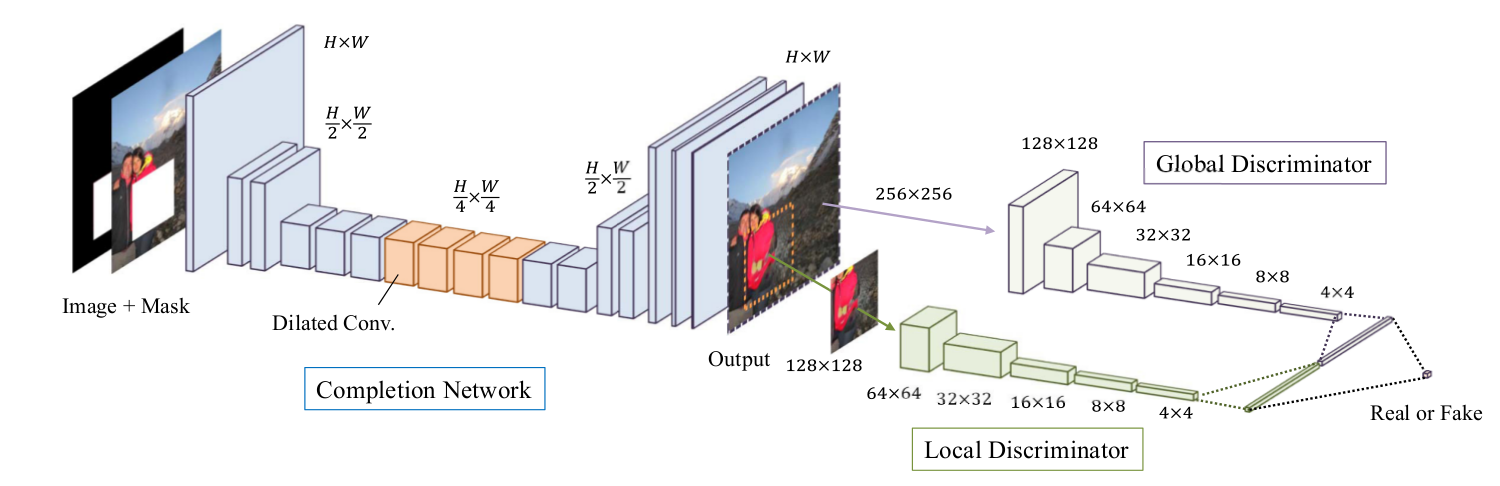
\includegraphics[width=1.0\textwidth]{Images/network_overview.png}
    \caption{Overview of the architecture}
\end{figure}

\subsection{Entrainement}

\section{Observation sur des exemples}

\subsection{Dataset utilisé pour entrainement : Places2}

Tout d'abord, on peut réutiliser des images appartenant au dataset de validation de Places2. Bien que les images soient diverses, on obtient des résultats corrects pour les images de paysages, même s'ils ne sont pas toujours satisfaisants pour de l'inpainting de visages (cf. section ci-dessous).

IMAGES

--Discussion des images--

\subsection{Différentes formes de masks}

L'entraînement du réseau s'est fait en utilisant des masks rectangulaires. Il nous semblait donc possible que l'inpainting sera moins performant si l'on utilise des masks moins réguliers. Pour tester cette hypothèse, nous avons comparé les résultats obtenus sur la même image, en cachant le même objet, mais avec des masks différents.

IMAGES

--Discussion des images--

\subsection{Visage (CelebA)}

Un autre point que nous avons voulu tester est l'inpainting sur les visages. En théorie, la méthode utilisant de l'apprentissage profond fonctionne mieux que la mathode par patchs pour compléter des visages, car il est souvent nécessaire d'inventer de nouveaux objets comme des yeux, un nez, des cheveux, etc. et la mathode par patch n'a possiblement pas ces objets en réserve. Cependant, les tests que nous avons fait ne sont pas très concluant. En effet, pour obtenir les résultats présentés dans le papier, le réseau a été entraîné spécifiquement et nous ne disposons pas de cet autre réseau. A notre grande déception, ce modele n'est pas disponible pour faire des test.

IMMAGE GITHUB

IMAGES TEST

--Discussion des images--

\subsection{Zero-Padding}

Le papier stipule que les maks qui sont trop près du bord ne donnent pas de bons résultats. Pour vérifier cette affirmation, nous avons effectué plusieurs tests avec des masks plus ou moins près du bord, sur la même image.

\begin{figure}[H]
    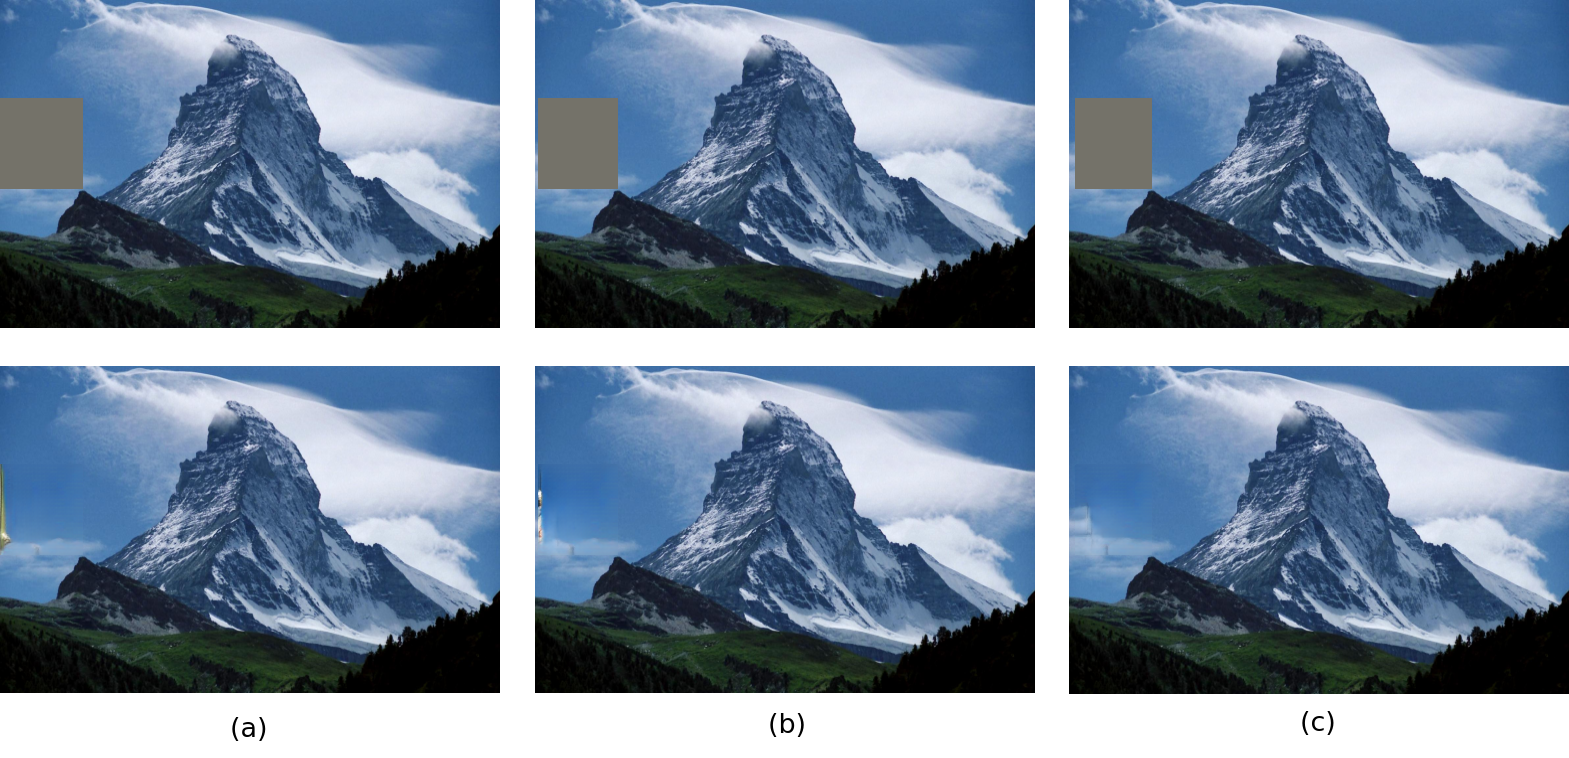
\includegraphics[width=1.0\textwidth]{Images/padding.png}
    \caption{(a), (b), (c) inputs et outputs (sans postprocess) à une distance de (a) 0 pixel, (b) 3 pixels, (c) 6 pixels du bord. Seul le cas (c) est convainquant, les autres ont des artefacts}
\end{figure}

Quand le mask est trop près du bord, on constate un artefact dû au fait qu l'on moyenne du noir (en dehors de l'image), ce qui ressort sur le côté. Cependant, dès que l'on est à une distance relativement faible du bord, le résultat n'est plus affecté par ce problème : s'il y a des artefacts, ce n'est plus dû à la trop grande proximité avec le bord.

\section{Bidouilles du réseau}



\subsection{Batchnormlisation}


\subsection{Rajouter du bruit dans les couches}

\subsubsection{Test avec une image de référence}
Test et observation de la dégradation de l'inpainting

\section{Questions additionnelles}

Il y a d'autres questions que nous nous sommes posées, mais il n'est pas possible avec nos moyens d'y répondre. Il est cependant intéressant de se les poser pour avoir une vue plus globale sur le papier.
\begin{itemize}
    \item a quel point le réseau fait-il du surapprentissage lorsque l'on l'entraîne spécifiquement (sur des visages par exemple) ?
    \item est-ce que la complétion vient d'un "patch" retenu lors de l'entraînement ou bien est-ce qu'elle est créée ?
\end{itemize}

\section{Bonus}

\subsection{Test du réseau sur des images non naturelles}

Avec un style un peu différent.

\begin{figure}[H]
    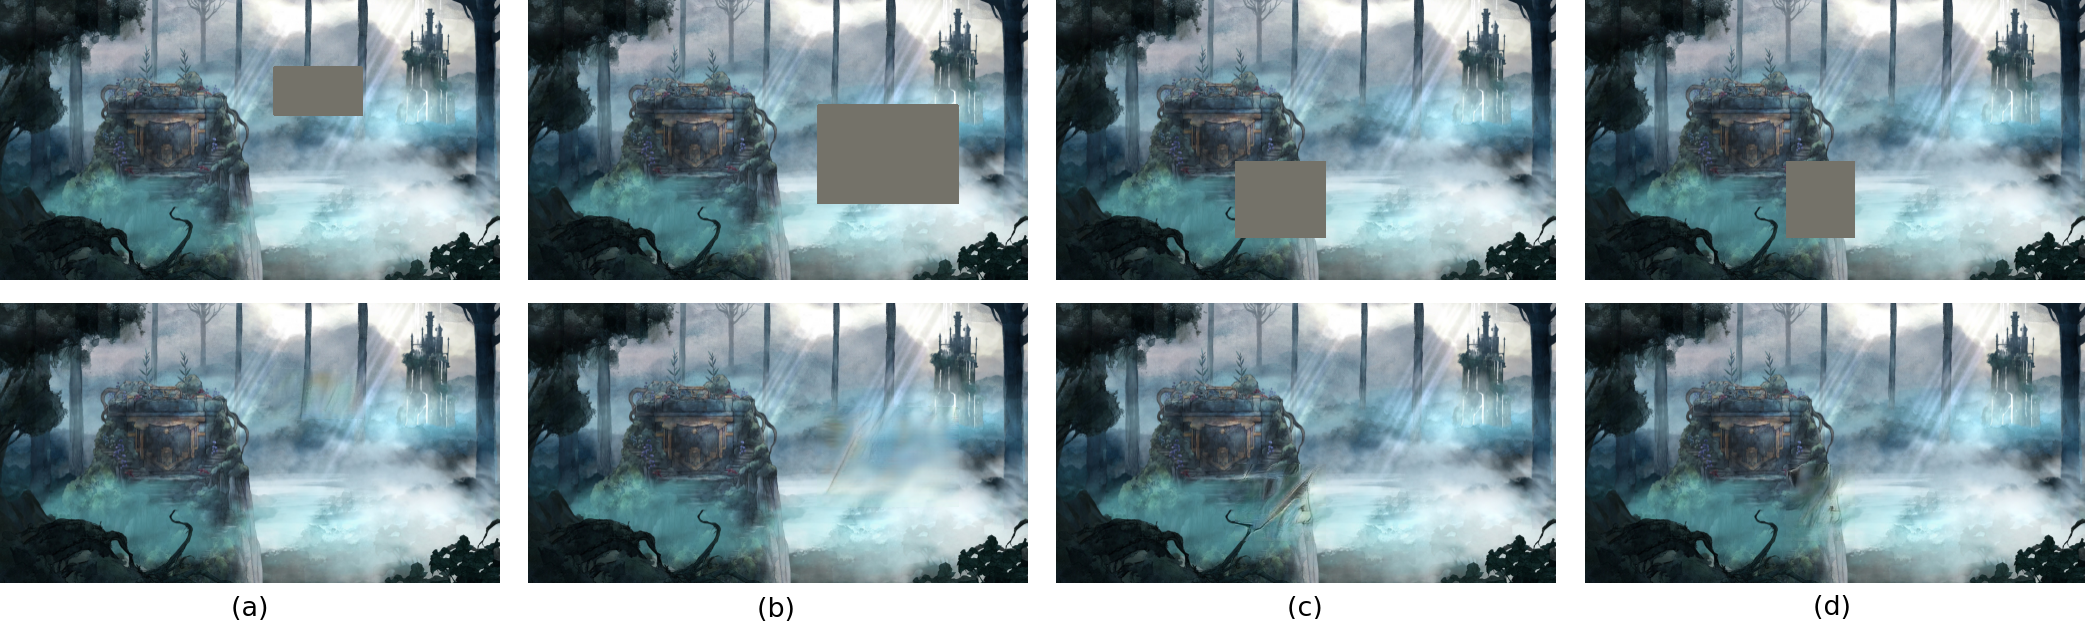
\includegraphics[width=1.0\textwidth]{Images/Col.png}
    \caption{(a), (b), (c) et (d) des inputs et outputs (sans postprocess) sur une image ayant un style particulier (type pastel).}
\end{figure}

Sur un style qui diffère un peu, mais pas de manière trop brutale avec les images naturelles qui composent en immense majorité Places2 (il n'est pas exclu qu'il y ait des images de pastels), on obtient un résultat qui contient parfois des artefacts, mais qui est parfois convainquant, ce qui est plutôt une bonne surprise.

Avec un style très particulier.

\begin{figure}[H]
    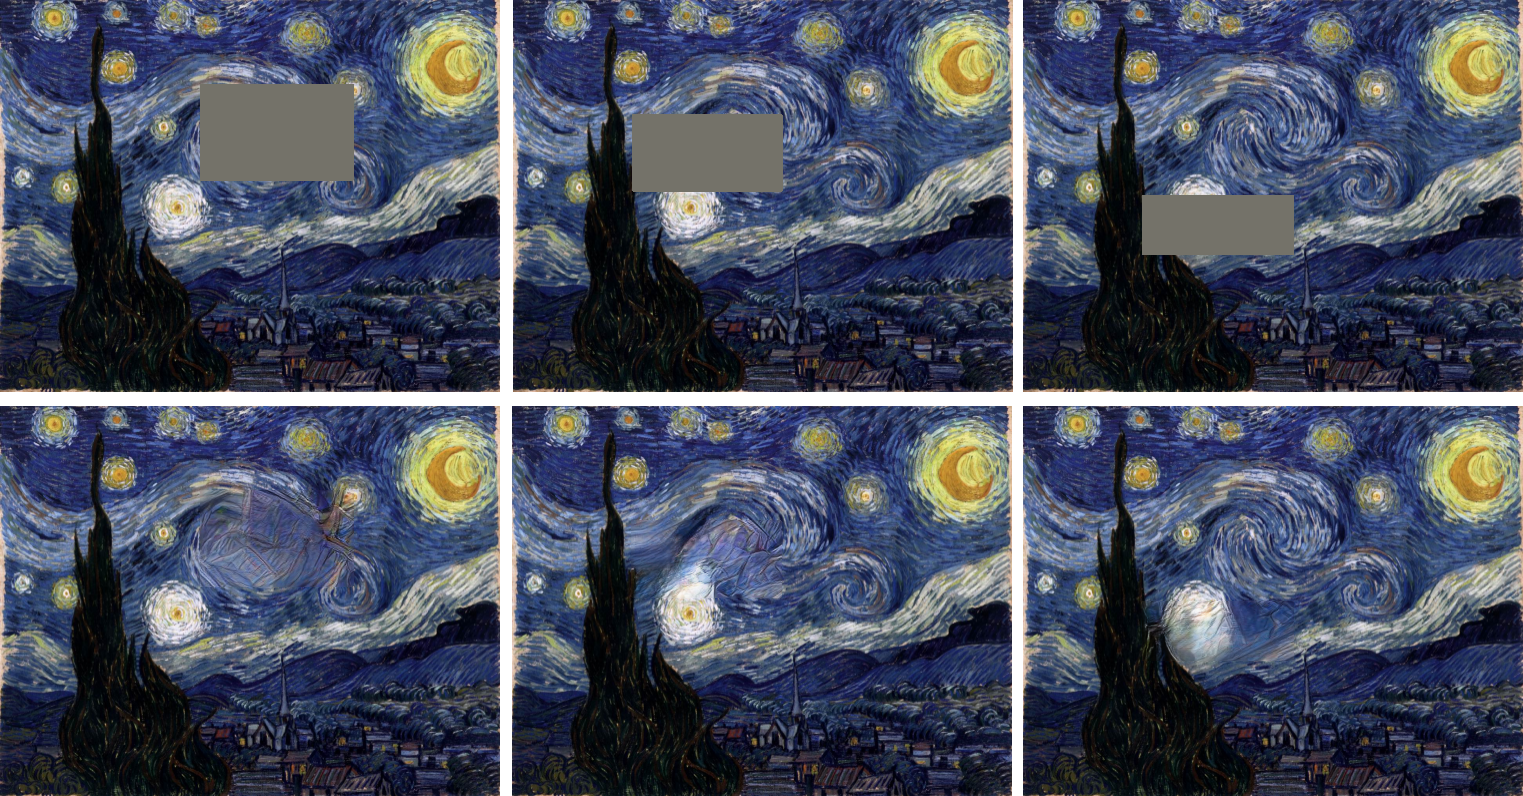
\includegraphics[width=1.0\textwidth]{Images/gogh.png}
    \caption{Inpainting (sans postprocess) de la nuit étoilée de Van Gogh.}
\end{figure}

Comme on pouvait s'y attendre, le réseau à beaucoup de mal à s'adapter au style d'une image particulière. La complétion n'est pas abérrente en soi (localement), mais elle ne s'accorde pas avec le style global de l'image.

\bibliographystyle{plain}
\bibliography{bib}

\end{document}
